\section{Theory}
\subsection{Linear Beam Optics}
In order to simulate the storage ring, we are using linear beam optics as described in [5]. However we are using a 6 dimensional model there and not a 4 dimensional model as described there. Our transformation matrix for a combined function magnet is given by:
\begin{equation} M = \left( \begin{array}{cccccc}
\cos \phi_x & \frac \rho {\sqrt{1 - n}} \sin \phi_x & 0 & 0 & 0 & \frac \rho {1 - n} (1 - \cos \phi_x) \\
- \frac{\sqrt{1 - n}} \rho \sin \phi_x & \cos \phi_x & 0 & 0 & 0 & \frac 1 {\sqrt{1 - n}} \sin \phi_x \\
0 & 0 & \cos \phi_y & \frac \rho n \sin \phi_y & 0 & 0 \\
0 & 0 & - \frac {\sqrt n} \rho \sin \phi_x & \cos \phi_x & 0 & 0 \\
- \frac 1 {\sqrt{1 - n}} \sin \phi_x & - \frac \rho {1- n } (1 - \cos \phi_x) & 0 & 0 & 1 & \frac \rho {(1 - n)^{3/2}} - \frac L {1 - n} \\
0 & 0 & 0 & 0 & 0 & 1 \end{array} \right) \end{equation}
with $\phi_x = \rho \sqrt{1 - n}$, $\phi_y = \phi \sqrt n$ and $L = \phi \cdot \rho$, where $\rho$ is the radius of the magnet, $\phi$ is the angle and n the field index.\\
Our cavity matrix is given by:
\begin{equation} M = \left( \begin{array}{cccccc}
1 & 0 & 0 & 0 & 0 & 0 \\
0 & 1 & 0 & 0 & 0 & 0 \\
0 & 0 & 1 & 0 & 0 & 0 \\
0 & 0 & 0 & 1 & 0 & 0 \\
0 & 0 & 0 & 0 & 1 & 0 \\
0 & 0 & 0 & 0 & \frac {\Delta E} E & 1 
\end{array} \right). \end{equation}
Where we have:
\begin{equation} \frac{\Delta E} E = \frac{2 \pi e V \cos \phi_s}{E \lambda} \end{equation}
where $\phi_s$ is the phase.
\subsection{Beam Matching}
To do the matching we proceed as follows. We have the linear map:
\begin{equation}
\left( \begin{array}{c}z \\ z' \end{array} \right)_f =
\left( \begin{array}{cc} A & B \\ C & D \end{array} \right) \cdot
\left( \begin{array}{c}z \\ z' \end{array} \right)_i .
\end{equation}
We then put:
\begin{equation}
\left( \begin{array}{cc} A & B \\ C & D \end{array} \right) =
\left( \begin{array}{cc} \cos \mu_s & - \beta_s \sin \mu_s \\ 
\frac 1 {\beta_s} \sin \mu_s & \cos \mu_s \end{array} \right).
\end{equation}
And we get the standard deviations of the beam with:
\begin{eqnarray} \sigma_z &=& \sqrt{\epsilon_z \beta_z} \textnormal{ and}\\
\sigma_{z'} &=& \sqrt{\frac{\epsilon_z}{\beta_z}}.
\end{eqnarray}
Something similar should work for the x and y direction. The transformation matrix is the one for the whole storage ring, the one turn map. See [5] for more information.

\subsection{Debye Length}
In approximations we often need a characteristic length. For this we can use the Debye Length, given by:
\begin{equation} \lambda_D = \left(\frac{\epsilon_0 k_B T}{q^2 n} \right)^2 \end{equation}
where T is the temperature, q the charge and n the density. In the theory of plasmas (and also for nonneutral plasmas) the Coulomb potential is shielded, if 2 electrons are farther apart then $\lambda_D$.\\
For more Information on the Debye Length see [1] Section 3.4 page 59 or [2] begins of chapter 4 page 186.\\
When we were doing particle - particle interactions we restricted our self to interactions where the distance was smaller, then the Debye length.

\subsubsection{Temperature of a relativistic beam}
In our formula for the Debye Length $\lambda_D$, it is not clear what the temperature is. Actually for our beam we have several temperatures, like the transversal and longitudinal temperatures. We also need to pay attention to in which frame we compute the temperature. However the beam is much smaller in the transversal direction, then in the longitudinal directions. Especially since by transforming to the beam frame, the beam becomes bigger by a factor of $\gamma$ in the longitudinal direction. So we can take the transversal temperature, which is given by:
\begin{equation} k_B T = m \overline{v_\perp ^2} \end{equation}
in the beam frame. To transform into the laboratory frame, the m goes to $\gamma m$.

\subsection{Relativistic considerations and effects}
In our simulation we use 3 frames of reference. One is the laboratory frame, one is the beam or bunch frame and one is the center of momentum frame. The laboratory frame is moving with the beam, so turning around with it, and moving. The beam frame is the one where the reference particle is at rest. So the difference between these 2 is a Lorentz transformation with the beam velocity in transversal direction to the beam.\\
The center of momentum frame is always different for the particles. In it the center of mass of the 2 particles is at rest, so they are only in relative motion, with speeds opposite to each other. This is for example necessary to compute the cross section.

\subsubsection{Lorentz Transformation}
To pass from the laboratory frame to beam frame, we have to use the Lorentz transformation, so we have:
\begin{eqnarray}
\beta &=& \frac v c \\
\gamma &=& \left(1 - \beta^2\right)^{-1/2}
\end{eqnarray}
\begin{equation}
\left(\begin{array}{c}t\\x\\y\\s \end{array}\right)_B =
\left( \begin{array}{cccc}
\gamma & 0 & 0 & - \beta \gamma \\ 
0 & 1 & 0 & 0 \\ 
0 & 0 & 1 & 0 \\ 
- \beta \gamma & 0 & 0 & \gamma 
\end{array} \right) 
\cdot \left(\begin{array}{c}t\\x\\y\\s\end{array} \right)_L.
\end{equation}
This mainly leads to the bunch become larger by a factor of $\gamma$ in the beam frame. Also note, that the relativistic momentum is given by:
\begin{equation}
p = (\gamma m_0 c, \gamma m_0 v^1, \gamma m_0 v^2, \gamma m_0 v^3)
\end{equation}
and that it transforms like the coordinate, so:
\begin{equation} p_B = \Lambda \cdot p_L \end{equation}
with $\Lambda$ the 4 x 4 Matrix above.
\subsection{Momentum Coordinate and collision}
For the coordinates for the momentum we use relative unit less coordinates, so from the real momentum $p_z$ to our coordinate $z'$ we transform with:
\begin{equation} z' = \frac{p_z - p_{0}}{p_{0}} = \frac{p_z}{p_0} - 1 \end{equation}
where $p_{0}$ is a reference momentum in the z direction. Taken here as $p_{0} = \gamma m_0 \beta c$. For the transversal coordinates we have:
\begin{equation} x' = \frac{p_x}{p_0} \ , \ y' = \frac{p_y}{p_0} \ , \ p_0  = \gamma m_0 \beta c. \end{equation}
To do the collision only the longitudinal coordinate gets transformed by a Lorentz transformation so we have, with E the energy:
\begin{equation} (E, p) \rightarrow (E', p') = (\gamma E - \beta \gamma p, \gamma p - \beta \gamma E). \end{equation}
Then the collision leads to a momentum change by $\Delta p$, so we have:
\begin{equation} p' \rightarrow p' + \Delta p. \end{equation}
This gets back transformed into the laboratory system leading to:
\begin{equation} p_{new} = p + \gamma \Delta p = p_0 + z' \cdot p_0 + \gamma \Delta p.\end{equation}
So this would lead us to a change in the coordinate z' by
\begin{equation} z' \rightarrow z' + \frac{\gamma \Delta p}{p_0}. \end{equation}
Using that $\Delta p = m_0 \cdot \Delta v$ and $p_0 = \gamma m_0 \beta c$ we get:
\begin{equation} z' \rightarrow z' + \frac{\Delta v}{\beta c}. \end{equation}

\subsubsection{Why we need to be fully relativistic}
The relativistic speed is given by:
\begin{equation}u^i = \frac{dx^i}{d\tau}. \end{equation}
Where $\tau$ denotes the proper time. The momentum is then $p = m u$, so we get in the laboratory system: $p = \gamma m v$ where v is the velocity measured in the laboratory system. The x and y components of the velocity aren't transformed when passing to the beam system, so we still have the same there. Assuming we would be able to calculate using classical mechanics, we would have $p = m v$ so $v_B = m v_L$ with $v_L \approx 10^5 m / s$ we would run to speeds bigger then the speed of light, for $\gamma > 3000$, which is a more then realistic value where we want to do the calculations.

\subsection{Quantum Electrodynamics}
The cross section we are using for electron electron scattering comes from quantum electrodynamics, it is given by:
\begin{equation} \sigma = \frac{d\sigma}{d\Omega} = \frac{r_e ^2}{4} \left(1 - \frac{v^2}{c^2}\right) \left[ (X+1)^2 \left(\frac 4 {\sin^4 \Theta} - \frac 3 {\sin^2 \Theta}\right) + 1 + \frac 4 {\sin^2 \Theta}\right] \end{equation}
with
\begin{equation} X = \left(\frac c v\right)^2 = \beta^{-2} = \frac{\gamma^2}{\gamma^2 - 1}. \end{equation}
It is derived assuming that the scattering process is done by the exchange of one photon. This formula is called M{\o}ller-Scattering, because M{\o}ller was the first to derive it. For a derivation of this cross section consult [13].

\begin{figure}[here]
 \centering
 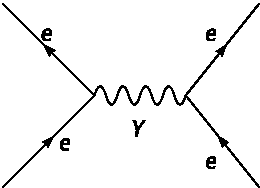
\includegraphics[width=0.50\textwidth]{inter.pdf}
 \caption{Feynman Diagram of the interaction}
\end{figure}


This cross section formula is valid in the center of momentum frame of both electrons.

\subsection{Analytical Touschek Effect}
There are some analytical results on the Touschek effect, so we have formulas for how many particles are left after a certain time. To compute this, one assumes the following:
\begin{equation}\frac{dN}{dt} = - \alpha N^2. \end{equation}
This is reasonable, because each particle has N possible particles to scatter of, so we got a total of $N^2$ of chances of a particle being lost. This leads to the function of particles in time, given by:
\begin{equation} N(t) = N_0 \cdot \frac 1 {1 + N_0 \alpha t} \end{equation}
with $N_0$ the number of particles at the time 0. The half lifetime is given by:
\begin{equation}\tau_{1/2} = - \frac{N(0)}{\dot N(0)} = \frac 1 {\alpha N(0)}. \end{equation}
\subsubsection{Classical Formula}
After Andreas Streun in [3], the factor $\alpha$ is given by:
\begin{equation} \alpha = \frac{r_0 ^2 c}{8 \pi \gamma^3 \sigma_s} \frac{F\left(\left(\frac{\delta_{acc}}{\gamma \sigma_{x'}}\right)^2\right)}{\sigma_x \sigma_y \sigma_{x'} \delta_{acc} ^2}. \end{equation}
  \begin{itemize}
  \item $r_0$ the classical electron radius.
  \item $\delta_{acc}$ the momentum acceptance.
  \item $\sigma_x$ the standard deviation of the bunch size.
  \item $\sigma_{x'} = \frac{\epsilon_x}{\sigma_x} \sqrt{1 + H \cdot \frac{\sigma_{t'} ^2}{\epsilon_x}}$ is the rms divergence of the $p / p_0$ at $x = 0.$
  \item $F(x) = \int\limits_0^1 \left(\frac 2 u - \ln \frac 1 u -2\right) e^{-x / u} du$
  \end{itemize}
\subsubsection{V\"olkel's Approach}  
Following Uta V\"olkel in [11] the parameter $\alpha$ for a gaussian distributed beam is given by:
\begin{eqnarray}
\alpha &=& \frac {4 \pi r_0 ^2 c}{V \Delta p_{max} ^2} \cdot J \\
J &=& \int\limits_\eta^{\delta p} \frac{\sqrt{1 + p_x ^2}}{p_x} \left(1 + \frac{p_x ^2}{1 + p_x ^2}\right)^2 F(p_x) d p_x - \frac 3 4 F(0) \\
F(p_x) &=& \frac{1}{2 \sqrt \pi \delta q} e^{- \left(\frac{p_x}{\delta q}\right)^2}. 
\end{eqnarray}
Here V is the volume of the bunch in the lab system. $\delta q$ is the rms of transverse momenta in units of $m_0 c$. This means that $\delta q \approx \gamma \sigma_{x'}$, and $\delta p$ is the maximal transverse momenta, given by $\delta p = \sqrt{3} \delta q$. $\Delta p_{max}$ is the momentum acceptance and $\eta = \Delta p_{max} / \gamma$.For more details see [11]. The 2 approaches at calculating the factor $\alpha$ gives about to the same result.

\subsection{Scattering at an angle}
Here we are following what S. Khan did in [10]. We want to scatter 2 electrons by the polar angle $\Theta$ and the azimuthal angle $\Phi$. Our electrons have the momenta in the laboratory frame:
\begin{equation} \vec p_{L} = \gamma m_0 \beta c (x', y', z' + 1).\end{equation}
We now first Lorentz transform this to the bunch system. Leading us to:
\begin{equation} p_{xB} = p_{xL},\ \ p_{yB} = p_{yL},\ \ p_{zB} = \gamma p_{zL} - \beta \gamma \sqrt{p_L ^2 + m_0^2 c^2}.\end{equation}
Till now  $\beta$ and $\gamma$ were used for the transformation from laboratory to the bunch system. Now, we will use them to transform from the bunch system into the center of mass system.\\
The energy of one electron is given by:
\begin{equation} E = \sqrt{ p ^2 c^2 + m_e ^2 c^4}. \end{equation}
It is different for the 2 electrons. The relativistic parameters to transform into the center of momenta system are given by:
\begin{equation} \vec \beta = \frac{\vec p_1 + \vec p_2}{E_1 + E_2} c \end{equation}
and we can obtain $\gamma$ by:
\begin{equation} \gamma = \frac 1 {\sqrt{1 - \beta^2}} \end{equation}
We have the transformation
\begin{equation} \vec q_i = \vec p_i + \vec \beta \gamma \left[ \frac \gamma {\gamma + 1} \vec \beta \vec p_i - \frac{E_i}{c}\right] \end{equation}
and the back transformation
\begin{equation} \vec \beta \rightarrow - \vec \beta  \end{equation}
and using the right energy $E = \sqrt{ p^2 c^2 + m_e ^2 c^4}$.\\

We rotate the vector $\vec q$ into the z direction, do the scattering and transform it back, so we have:
\begin{equation} \theta = \cos^{-1} \frac {q_z} q \ \ \phi = \frac \pi 2 + \tan^{-1} \frac {q_y}{q_x} \ \ \ \psi = 0. \end{equation}
We also need to consider, that in case of $q_z < 0$, $\theta \rightarrow \theta + \pi$.\\
And we get as a vector $\vec q'$ after the scattering:
\begin{equation} \vec q' = \left(\begin{array}{ccc}
\cos \phi & - \cos \theta \sin \phi & \sin \theta \sin \phi \\
\sin \phi & \cos \theta \cos \phi & - \sin \theta \sin \phi \\
0 & \sin \theta & \cos \theta \end{array} \right) \cdot q \cdot
\left( \begin{array}{c} \sin \Theta \cos \Phi \\ \sin \Theta \sin \Phi \\ \cos \Theta \end{array} \right) \end{equation}
where q denotes the length of the vector $\vec q$ before the collision.\\
We then apply the back transform (twice! first to the bunch, then to the lab) and check if we are outside the momentum acceptance.

\subsection{Idea behind the cross section}
The main idea behind the cross section is to solve the integral for the lost rate given by:
\begin{equation} \dot N = \frac 1 {\gamma C} \int\limits_0^C ds \\
\int\limits_{-\infty}^\infty dx dy dz \\
\int\limits_{-\infty}^\infty dx'_1 dy'_1 dz'_1 \\
\int\limits_{-\infty}^\infty dx'_2 dy'_2 dz'_2 \\
\int\limits_{4 \pi} d(\cos\Theta) d\Phi 2v \sigma \rho_1 \rho_2. \end{equation}
Here we are integrating over a 12 dimensional volume. $d(\cos \Theta) d\Phi = d\Theta d\Phi \sin \Theta$ is an area element in the angle coordinates. $\int_{-\infty}^\infty dx dy dz$ is the integration over all possible positions where the interaction could take place. $\int_{-\infty}^\infty dx'_1 dy'_1 dz'_1$ and $\int_{-\infty}^\infty dx'_2 dy'_2 dz'_2$ over the possible momenta of the 2 interaction partners. $\int_0^C ds$ is the integral along the storage ring, because the parameters before depend on where you are in the ring.
\subsection{Idea behind Monte Carlo Integration}
The idea behind Monte Carlo Integration is that, for n points $u_1, ..., u_n$ picked at random in the interval $\left[u, u + \Delta u\right]$, we have that:
\begin{equation} \int\limits_u^{u + \Delta u} f(u) du \approx \frac{\Delta u}{n} \sum\limits_{k=1}^n f(u_k). \end{equation}
This way we hope to solve our above integral, applying the same procedure to the multidimensional integral above. To be exact this is what Khan did in [4]. We are additionally adding in particle tracking.
